\documentclass[aspectratio=169]{beamer}

\usepackage[utf8]{inputenc}
\usetheme{Singapore}
\usepackage{xcolor}
\setbeamertemplate{footline}[frame number]

\usepackage{../sty/mathlist}   % provides the `algo' environment used below
\usepackage{amsmath,amssymb}

\usepackage{tikz}
\usetikzlibrary{positioning}

\usepackage{times}

\setbeamercovered{dynamic}

% We add the following commonly used macros:

\usepackage{graphicx}
\graphicspath{{../imgs/}{imgs/}{./}}


% vectors as boldsymbols:
\newcommand{\bsa}{{\boldsymbol{a}}}
\newcommand{\bsb}{{\boldsymbol{b}}}
\newcommand{\bsc}{{\boldsymbol{c}}}
\newcommand{\bsd}{{\boldsymbol{d}}}
\newcommand{\bse}{{\boldsymbol{e}}}
\newcommand{\bsf}{{\boldsymbol{f}}}
\newcommand{\bsg}{{\boldsymbol{g}}}
\newcommand{\bsh}{{\boldsymbol{h}}}
\newcommand{\bsi}{{\boldsymbol{i}}}
\newcommand{\bsj}{{\boldsymbol{j}}}
\newcommand{\bsk}{{\boldsymbol{k}}}
\newcommand{\bsl}{{\boldsymbol{l}}}
\newcommand{\bsm}{{\boldsymbol{m}}}
\newcommand{\bsn}{{\boldsymbol{n}}}
\newcommand{\bso}{{\boldsymbol{o}}}
\newcommand{\bsp}{{\boldsymbol{p}}}
\newcommand{\bsq}{{\boldsymbol{q}}}
\newcommand{\bsr}{{\boldsymbol{r}}}
\newcommand{\bss}{{\boldsymbol{s}}}
\newcommand{\bst}{{\boldsymbol{t}}}
\newcommand{\bsu}{{\boldsymbol{u}}}
\newcommand{\bsv}{{\boldsymbol{v}}}
\newcommand{\bsw}{{\boldsymbol{w}}}
\newcommand{\bsx}{{\boldsymbol{x}}}
\newcommand{\bsy}{{\boldsymbol{y}}}
\newcommand{\bsz}{{\boldsymbol{z}}}
\newcommand{\bsA}{{\boldsymbol{A}}}
\newcommand{\bsB}{{\boldsymbol{B}}}
\newcommand{\bsC}{{\boldsymbol{C}}}
\newcommand{\bsD}{{\boldsymbol{D}}}
\newcommand{\bsE}{{\boldsymbol{E}}}
\newcommand{\bsF}{{\boldsymbol{F}}}
\newcommand{\bsG}{{\boldsymbol{G}}}
\newcommand{\bsH}{{\boldsymbol{H}}}
\newcommand{\bsI}{{\boldsymbol{I}}}
\newcommand{\bsJ}{{\boldsymbol{J}}}
\newcommand{\bsK}{{\boldsymbol{K}}}
\newcommand{\bsL}{{\boldsymbol{L}}}
\newcommand{\bsM}{{\boldsymbol{M}}}
\newcommand{\bsN}{{\boldsymbol{N}}}
\newcommand{\bsO}{{\boldsymbol{O}}}
\newcommand{\bsP}{{\boldsymbol{P}}}
\newcommand{\bsQ}{{\boldsymbol{Q}}}
\newcommand{\bsR}{{\boldsymbol{R}}}
\newcommand{\bsS}{{\boldsymbol{S}}}
\newcommand{\bsT}{{\boldsymbol{T}}}
\newcommand{\bsU}{{\boldsymbol{U}}}
\newcommand{\bsV}{{\boldsymbol{V}}}
\newcommand{\bsW}{{\boldsymbol{W}}}
\newcommand{\bsX}{{\boldsymbol{X}}}
\newcommand{\bsY}{{\boldsymbol{Y}}}
\newcommand{\bsZ}{{\boldsymbol{Z}}}
% other commonly used boldsymbols:
\newcommand{\bsell}{{\boldsymbol{\ell}}}
\newcommand{\bszero}{{\boldsymbol{0}}} % vector of zeros
\newcommand{\bsone}{{\boldsymbol{1}}}  % vector of ones
% boldsymbol greeks:
\newcommand{\bsalpha}{{\boldsymbol{\alpha}}}
\newcommand{\bsbeta}{{\boldsymbol{\beta}}}
\newcommand{\bsgamma}{{\boldsymbol{\gamma}}}
\newcommand{\bsdelta}{{\boldsymbol{\delta}}}
\newcommand{\bsepsilon}{{\boldsymbol{\epsilon}}}
\newcommand{\bsvarepsilon}{{\boldsymbol{\varepsilon}}}
\newcommand{\bszeta}{{\boldsymbol{\zeta}}}
\newcommand{\bseta}{{\boldsymbol{\eta}}}
\newcommand{\bstheta}{{\boldsymbol{\theta}}}
\newcommand{\bsvartheta}{{\boldsymbol{\vartheta}}}
\newcommand{\bskappa}{{\boldsymbol{\kappa}}}
\newcommand{\bslambda}{{\boldsymbol{\lambda}}}
\newcommand{\bsmu}{{\boldsymbol{\mu}}}
\newcommand{\bsnu}{{\boldsymbol{\nu}}}
\newcommand{\bsxi}{{\boldsymbol{\xi}}}
\newcommand{\bspi}{{\boldsymbol{\pi}}}
\newcommand{\bsvarpi}{{\boldsymbol{\varpi}}}
\newcommand{\bsrho}{{\boldsymbol{\rho}}}
\newcommand{\bsvarrho}{{\boldsymbol{\varrho}}}
\newcommand{\bssigma}{{\boldsymbol{\sigma}}}
\newcommand{\bsvarsigma}{{\boldsymbol{\varsigma}}}
\newcommand{\bstau}{{\boldsymbol{\tau}}}
\newcommand{\bsupsilon}{{\boldsymbol{\upsilon}}}
\newcommand{\bsphi}{{\boldsymbol{\phi}}}
\newcommand{\bsvarphi}{{\boldsymbol{\varphi}}}
\newcommand{\bschi}{{\boldsymbol{\chi}}}
\newcommand{\bspsi}{{\boldsymbol{\psi}}}
\newcommand{\bsomega}{{\boldsymbol{\omega}}}
\newcommand{\bsGamma}{{\boldsymbol{\Gamma}}}
\newcommand{\bsDelta}{{\boldsymbol{\Delta}}}
\newcommand{\bsTheta}{{\boldsymbol{\Theta}}}
\newcommand{\bsLambda}{{\boldsymbol{\Lambda}}}
\newcommand{\bsXi}{{\boldsymbol{\Xi}}}
\newcommand{\bsPi}{{\boldsymbol{\Pi}}}
\newcommand{\bsSigma}{{\boldsymbol{\Sigma}}}
\newcommand{\bsUpsilon}{{\boldsymbol{\Upsilon}}}
\newcommand{\bsPhi}{{\boldsymbol{\Phi}}}
\newcommand{\bsPsi}{{\boldsymbol{\Psi}}}
\newcommand{\bsOmega}{{\boldsymbol{\Omega}}}

% Roman fonts:
\newcommand{\rma}{{\mathrm{a}}}
\newcommand{\rmb}{{\mathrm{b}}}
\newcommand{\rmc}{{\mathrm{c}}}
\newcommand{\rmd}{{\mathrm{d}}}
\newcommand{\rme}{{\mathrm{e}}}
\newcommand{\rmf}{{\mathrm{f}}}
\newcommand{\rmg}{{\mathrm{g}}}
\newcommand{\rmh}{{\mathrm{h}}}
\newcommand{\rmi}{{\mathrm{i}}}
\newcommand{\rmj}{{\mathrm{j}}}
\newcommand{\rmk}{{\mathrm{k}}}
\newcommand{\rml}{{\mathrm{l}}}
\newcommand{\rmm}{{\mathrm{m}}}
\newcommand{\rmn}{{\mathrm{n}}}
\newcommand{\rmo}{{\mathrm{o}}}
\newcommand{\rmp}{{\mathrm{p}}}
\newcommand{\rmq}{{\mathrm{q}}}
\newcommand{\rmr}{{\mathrm{r}}}
\newcommand{\rms}{{\mathrm{s}}}
\newcommand{\rmt}{{\mathrm{t}}}
\newcommand{\rmu}{{\mathrm{u}}}
\newcommand{\rmv}{{\mathrm{v}}}
\newcommand{\rmw}{{\mathrm{w}}}
\newcommand{\rmx}{{\mathrm{x}}}
\newcommand{\rmy}{{\mathrm{y}}}
\newcommand{\rmz}{{\mathrm{z}}}
\newcommand{\rmA}{{\mathrm{A}}}
\newcommand{\rmB}{{\mathrm{B}}}
\newcommand{\rmC}{{\mathrm{C}}}
\newcommand{\rmD}{{\mathrm{D}}}
\newcommand{\rmE}{{\mathrm{E}}}
\newcommand{\rmF}{{\mathrm{F}}}
\newcommand{\rmG}{{\mathrm{G}}}
\newcommand{\rmH}{{\mathrm{H}}}
\newcommand{\rmI}{{\mathrm{I}}}
\newcommand{\rmJ}{{\mathrm{J}}}
\newcommand{\rmK}{{\mathrm{K}}}
\newcommand{\rmL}{{\mathrm{L}}}
\newcommand{\rmM}{{\mathrm{M}}}
\newcommand{\rmN}{{\mathrm{N}}}
\newcommand{\rmO}{{\mathrm{O}}}
\newcommand{\rmP}{{\mathrm{P}}}
\newcommand{\rmQ}{{\mathrm{Q}}}
\newcommand{\rmR}{{\mathrm{R}}}
\newcommand{\rmS}{{\mathrm{S}}}
\newcommand{\rmT}{{\mathrm{T}}}
\newcommand{\rmU}{{\mathrm{U}}}
\newcommand{\rmV}{{\mathrm{V}}}
\newcommand{\rmW}{{\mathrm{W}}}
\newcommand{\rmX}{{\mathrm{X}}}
\newcommand{\rmY}{{\mathrm{Y}}}
\newcommand{\rmZ}{{\mathrm{Z}}}
% also commonly defined
\newcommand{\rd}{{\mathrm{d}}}
\newcommand{\ri}{{\mathrm{i}}}

% blackboards:
\newcommand{\bbA}{{\mathbb{A}}}
\newcommand{\bbB}{{\mathbb{B}}}
\newcommand{\bbC}{{\mathbb{C}}}
\newcommand{\bbD}{{\mathbb{D}}}
\newcommand{\bbE}{{\mathbb{E}}}
\newcommand{\bbF}{{\mathbb{F}}}
\newcommand{\bbG}{{\mathbb{G}}}
\newcommand{\bbH}{{\mathbb{H}}}
\newcommand{\bbI}{{\mathbb{I}}}
\newcommand{\bbJ}{{\mathbb{J}}}
\newcommand{\bbK}{{\mathbb{K}}}
\newcommand{\bbL}{{\mathbb{L}}}
\newcommand{\bbM}{{\mathbb{M}}}
\newcommand{\bbN}{{\mathbb{N}}}
\newcommand{\bbO}{{\mathbb{O}}}
\newcommand{\bbP}{{\mathbb{P}}}
\newcommand{\bbQ}{{\mathbb{Q}}}
\newcommand{\bbR}{{\mathbb{R}}}
\newcommand{\bbS}{{\mathbb{S}}}
\newcommand{\bbT}{{\mathbb{T}}}
\newcommand{\bbU}{{\mathbb{U}}}
\newcommand{\bbV}{{\mathbb{V}}}
\newcommand{\bbW}{{\mathbb{W}}}
\newcommand{\bbX}{{\mathbb{X}}}
\newcommand{\bbY}{{\mathbb{Y}}}
\newcommand{\bbZ}{{\mathbb{Z}}}
% commonly used shortcuts:
\newcommand{\C}{{\mathbb{C}}} % complex numbers
\newcommand{\F}{{\mathbb{F}}} % field, finite field
\newcommand{\N}{{\mathbb{N}}} % natural numbers {1, 2, ...}
\newcommand{\Q}{{\mathbb{Q}}} % rationals
\newcommand{\R}{{\mathbb{R}}} % reals
\newcommand{\Z}{{\mathbb{Z}}} % integers
% more commonly used shortcuts:
\newcommand{\CC}{{\mathbb{C}}} % complex numbers
\newcommand{\FF}{{\mathbb{F}}} % field, finite field
\newcommand{\NN}{{\mathbb{N}}} % natural numbers {1, 2, ...}
\newcommand{\QQ}{{\mathbb{Q}}} % rationals
\newcommand{\RR}{{\mathbb{R}}} % reals
\newcommand{\ZZ}{{\mathbb{Z}}} % integers
% more commonly used shortcuts:
\newcommand{\EE}{{\mathbb{E}}}
\newcommand{\PP}{{\mathbb{P}}}
\newcommand{\TT}{{\mathbb{T}}}
\newcommand{\VV}{{\mathbb{V}}}
% and even more commonly used shortcuts:
\newcommand{\Complex}{{\mathbb{C}}}
\newcommand{\Integer}{{\mathbb{Z}}}
\newcommand{\Natural}{{\mathbb{N}}}
\newcommand{\Rational}{{\mathbb{Q}}}
\newcommand{\Real}{{\mathbb{R}}}

%%% Issue with miktex
% indicator boldface 1:
%\DeclareSymbolFont{bbold}{U}{bbold}{m}{n}
%\DeclareSymbolFontAlphabet{\mathbbold}{bbold}
%\newcommand{\ind}{{\mathbbold{1}}}
%\newcommand{\bbone}{{\mathbbold{1}}}


% calligraphic letters:
\newcommand{\cala}{{\mathcal{a}}}
\newcommand{\calb}{{\mathcal{b}}}
\newcommand{\calc}{{\mathcal{c}}}
\newcommand{\cald}{{\mathcal{d}}}
\newcommand{\cale}{{\mathcal{e}}}
\newcommand{\calf}{{\mathcal{f}}}
\newcommand{\calg}{{\mathcal{g}}}
\newcommand{\calh}{{\mathcal{h}}}
\newcommand{\cali}{{\mathcal{i}}}
\newcommand{\calj}{{\mathcal{j}}}
\newcommand{\calk}{{\mathcal{k}}}
\newcommand{\call}{{\mathcal{l}}}
\newcommand{\calm}{{\mathcal{m}}}
\newcommand{\caln}{{\mathcal{n}}}
\newcommand{\calo}{{\mathcal{o}}}
\newcommand{\calp}{{\mathcal{p}}}
\newcommand{\calq}{{\mathcal{q}}}
\newcommand{\calr}{{\mathcal{r}}}
\newcommand{\cals}{{\mathcal{s}}}
\newcommand{\calt}{{\mathcal{t}}}
\newcommand{\calu}{{\mathcal{u}}}
\newcommand{\calv}{{\mathcal{v}}}
\newcommand{\calw}{{\mathcal{w}}}
\newcommand{\calx}{{\mathcal{x}}}
\newcommand{\caly}{{\mathcal{y}}}
\newcommand{\calz}{{\mathcal{z}}}
\newcommand{\calA}{{\mathcal{A}}}
\newcommand{\calB}{{\mathcal{B}}}
\newcommand{\calC}{{\mathcal{C}}}
\newcommand{\calD}{{\mathcal{D}}}
\newcommand{\calE}{{\mathcal{E}}}
\newcommand{\calF}{{\mathcal{F}}}
\newcommand{\calG}{{\mathcal{G}}}
\newcommand{\calH}{{\mathcal{H}}}
\newcommand{\calI}{{\mathcal{I}}}
\newcommand{\calJ}{{\mathcal{J}}}
\newcommand{\calK}{{\mathcal{K}}}
\newcommand{\calL}{{\mathcal{L}}}
\newcommand{\calM}{{\mathcal{M}}}
\newcommand{\calN}{{\mathcal{N}}}
\newcommand{\calO}{{\mathcal{O}}}
\newcommand{\calP}{{\mathcal{P}}}
\newcommand{\calQ}{{\mathcal{Q}}}
\newcommand{\calR}{{\mathcal{R}}}
\newcommand{\calS}{{\mathcal{S}}}
\newcommand{\calT}{{\mathcal{T}}}
\newcommand{\calU}{{\mathcal{U}}}
\newcommand{\calV}{{\mathcal{V}}}
\newcommand{\calW}{{\mathcal{W}}}
\newcommand{\calX}{{\mathcal{X}}}
\newcommand{\calY}{{\mathcal{Y}}}
\newcommand{\calZ}{{\mathcal{Z}}}

% Euler fraks:
\newcommand{\fraka}{{\mathfrak{a}}}
\newcommand{\frakb}{{\mathfrak{b}}}
\newcommand{\frakc}{{\mathfrak{c}}}
\newcommand{\frakd}{{\mathfrak{d}}}
\newcommand{\frake}{{\mathfrak{e}}}
\newcommand{\frakf}{{\mathfrak{f}}}
\newcommand{\frakg}{{\mathfrak{g}}}
\newcommand{\frakh}{{\mathfrak{h}}}
\newcommand{\fraki}{{\mathfrak{i}}}
\newcommand{\frakj}{{\mathfrak{j}}}
\newcommand{\frakk}{{\mathfrak{k}}}
\newcommand{\frakl}{{\mathfrak{l}}}
\newcommand{\frakm}{{\mathfrak{m}}}
\newcommand{\frakn}{{\mathfrak{n}}}
\newcommand{\frako}{{\mathfrak{o}}}
\newcommand{\frakp}{{\mathfrak{p}}}
\newcommand{\frakq}{{\mathfrak{q}}}
\newcommand{\frakr}{{\mathfrak{r}}}
\newcommand{\fraks}{{\mathfrak{s}}}
\newcommand{\frakt}{{\mathfrak{t}}}
\newcommand{\fraku}{{\mathfrak{u}}}
\newcommand{\frakv}{{\mathfrak{v}}}
\newcommand{\frakw}{{\mathfrak{w}}}
\newcommand{\frakx}{{\mathfrak{x}}}
\newcommand{\fraky}{{\mathfrak{y}}}
\newcommand{\frakz}{{\mathfrak{z}}}
\newcommand{\frakA}{{\mathfrak{A}}}
\newcommand{\frakB}{{\mathfrak{B}}}
\newcommand{\frakC}{{\mathfrak{C}}}
\newcommand{\frakD}{{\mathfrak{D}}}
\newcommand{\frakE}{{\mathfrak{E}}}
\newcommand{\frakF}{{\mathfrak{F}}}
\newcommand{\frakG}{{\mathfrak{G}}}
\newcommand{\frakH}{{\mathfrak{H}}}
\newcommand{\frakI}{{\mathfrak{I}}}
\newcommand{\frakJ}{{\mathfrak{J}}}
\newcommand{\frakK}{{\mathfrak{K}}}
\newcommand{\frakL}{{\mathfrak{L}}}
\newcommand{\frakM}{{\mathfrak{M}}}
\newcommand{\frakN}{{\mathfrak{N}}}
\newcommand{\frakO}{{\mathfrak{O}}}
\newcommand{\frakP}{{\mathfrak{P}}}
\newcommand{\frakQ}{{\mathfrak{Q}}}
\newcommand{\frakR}{{\mathfrak{R}}}
\newcommand{\frakS}{{\mathfrak{S}}}
\newcommand{\frakT}{{\mathfrak{T}}}
\newcommand{\frakU}{{\mathfrak{U}}}
\newcommand{\frakV}{{\mathfrak{V}}}
\newcommand{\frakW}{{\mathfrak{W}}}
\newcommand{\frakX}{{\mathfrak{X}}}
\newcommand{\frakY}{{\mathfrak{Y}}}
\newcommand{\frakZ}{{\mathfrak{Z}}}
% sets as Euler fraks:
\newcommand{\seta}{{\mathfrak{a}}}
\newcommand{\setb}{{\mathfrak{b}}}
\newcommand{\setc}{{\mathfrak{c}}}
\newcommand{\setd}{{\mathfrak{d}}}
\newcommand{\sete}{{\mathfrak{e}}}
\newcommand{\setf}{{\mathfrak{f}}}
\newcommand{\setg}{{\mathfrak{g}}}
\newcommand{\seth}{{\mathfrak{h}}}
\newcommand{\seti}{{\mathfrak{i}}}
\newcommand{\setj}{{\mathfrak{j}}}
\newcommand{\setk}{{\mathfrak{k}}}
\newcommand{\setl}{{\mathfrak{l}}}
\newcommand{\setm}{{\mathfrak{m}}}
\newcommand{\setn}{{\mathfrak{n}}}
\newcommand{\seto}{{\mathfrak{o}}}
\newcommand{\setp}{{\mathfrak{p}}}
\newcommand{\setq}{{\mathfrak{q}}}
\newcommand{\setr}{{\mathfrak{r}}}
\newcommand{\sets}{{\mathfrak{s}}}
\newcommand{\sett}{{\mathfrak{t}}}
\newcommand{\setu}{{\mathfrak{u}}}
\newcommand{\setv}{{\mathfrak{v}}}
\newcommand{\setw}{{\mathfrak{w}}}
\newcommand{\setx}{{\mathfrak{x}}}
\newcommand{\sety}{{\mathfrak{y}}}
\newcommand{\setz}{{\mathfrak{z}}}
\newcommand{\setA}{{\mathfrak{A}}}
\newcommand{\setB}{{\mathfrak{B}}}
\newcommand{\setC}{{\mathfrak{C}}}
\newcommand{\setD}{{\mathfrak{D}}}
\newcommand{\setE}{{\mathfrak{E}}}
\newcommand{\setF}{{\mathfrak{F}}}
\newcommand{\setG}{{\mathfrak{G}}}
\newcommand{\setH}{{\mathfrak{H}}}
\newcommand{\setI}{{\mathfrak{I}}}
\newcommand{\setJ}{{\mathfrak{J}}}
\newcommand{\setK}{{\mathfrak{K}}}
\newcommand{\setL}{{\mathfrak{L}}}
\newcommand{\setM}{{\mathfrak{M}}}
\newcommand{\setN}{{\mathfrak{N}}}
\newcommand{\setO}{{\mathfrak{O}}}
\newcommand{\setP}{{\mathfrak{P}}}
\newcommand{\setQ}{{\mathfrak{Q}}}
\newcommand{\setR}{{\mathfrak{R}}}
\newcommand{\setS}{{\mathfrak{S}}}
\newcommand{\setT}{{\mathfrak{T}}}
\newcommand{\setU}{{\mathfrak{U}}}
\newcommand{\setV}{{\mathfrak{V}}}
\newcommand{\setW}{{\mathfrak{W}}}
\newcommand{\setX}{{\mathfrak{X}}}
\newcommand{\setY}{{\mathfrak{Y}}}
\newcommand{\setZ}{{\mathfrak{Z}}}

% other commonly defined commands:
\newcommand{\wal}{{\rm wal}}
\newcommand{\floor}[1]{\left\lfloor #1 \right\rfloor} % floor
\newcommand{\ceil}[1]{\left\lceil #1 \right\rceil}    % ceil
\DeclareMathOperator{\cov}{Cov}
\DeclareMathOperator{\var}{Var}
\providecommand{\argmin}{\operatorname*{argmin}}
\providecommand{\argmax}{\operatorname*{argmax}}

% Colour switches inherited from PSTricks ({\red ...}, {\blue ...}).
% Defined here so that decks no longer need to load pstricks just for them.
\providecommand{\red}{\color{red}}
\providecommand{\blue}{\color{blue}}


\def\aff{\operatorname{aff}}
\def\cS{\mathcal{S}}
\def\cX{\mathcal{X}}


%% ---------------------------------------------------------------------------
%% Nonanticipativity pictures, in TikZ (no PSTricks, no auto-pst-pdf).
%% ---------------------------------------------------------------------------

% One root branching directly into the four scenarios.
\newcommand{\scenariofan}{%
  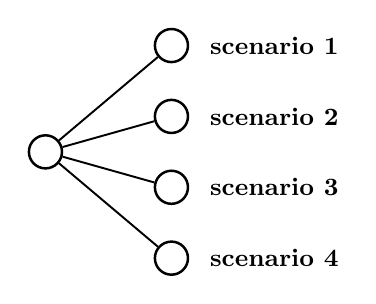
\begin{tikzpicture}[
      nd/.style={circle,draw,line width=0.9pt,minimum size=4.2mm,inner sep=0pt}]
    \node[nd] (r) at (0,0) {};
    \foreach \k/\y in {1/1.35,2/0.45,3/-0.45,4/-1.35} {
      \node[nd] (s\k) at (1.6,\y) {};
      \draw[line width=0.7pt] (r) -- (s\k);
      \node[font=\small\bfseries,right=4pt] at (s\k.east) {scenario \k};
    }
  \end{tikzpicture}}

% The same four scenarios as two periods of decision variables, the doubled
% bars marking the first-period copies that nonanticipativity ties together.
\newcommand{\scenariobundles}{%
  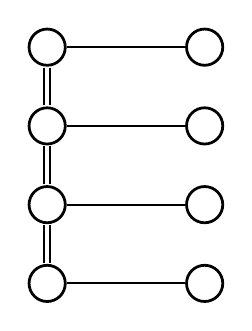
\begin{tikzpicture}[
      nd/.style={circle,draw,line width=1pt,minimum size=4.6mm,inner sep=0pt}]
    \foreach \r in {0,1,2,3} {
      \node[nd] (a\r) at (0,\r) {};
      \node[nd] (b\r) at (2,\r) {};
      \draw[line width=0.7pt] (a\r) -- (b\r);
    }
    \foreach \r/\rr in {3/2,2/1,1/0} {
      \draw[line width=0.7pt] (-0.04,\r-0.26) -- (-0.04,\rr+0.26);
      \draw[line width=0.7pt] ( 0.04,\r-0.26) -- ( 0.04,\rr+0.26);
    }
  \end{tikzpicture}}

\title[Stochastic Lagrangian]{Stochastic programming\\Lagrangian methods}

\author[Fabian Bastin]{Fabian Bastin \\ \texorpdfstring{\url{fabian.bastin@umontreal.ca}}{fabian.bastin@umontreal.ca} \\ Université de Montréal -- CIRRELT -- IVADO}

\date{}

\setbeamertemplate{footline}[frame number]

\begin{document}

\frame{\titlepage}

\begin{frame}
\frametitle{Motivation}

{\red Reference}: Birge and Louveaux, Sections~3.4, 5.8 and 6.4.

\mbox{}

We consider the general {\blue two-stage nonlinear program}
\begin{align*}
\inf z\ &= f^1(x) + \calQ(x) \\
\mbox{s.t. } & g_i^1(x) \leq 0,\ i = 1,\ldots,m_1,
\end{align*}
where $\calQ(x) = \EE_{\bsxi}[Q(x,\bsxi)]$, and
\begin{align*}
Q(x,\xi) = \inf\ & f^2(y(\xi),\xi) \\
\mbox{s.t. } & b_i^2(x,\xi) + g_i^2(y(\xi), \xi) \leq 0,\ i = 1,\ldots,m_2.
\end{align*}

We assume that all functions $f^2(\cdot,\xi)$, $b_i^2(\cdot,\xi)$ and $g_i^2(\cdot,\xi)$ are continuous in the first argument for any given $\xi$, and measurable in $\xi$ for any fixed first argument. $\bsxi$ has finite second-order moments.

\end{frame}

%\begin{frame}
%\frametitle{Application to stochastic programming}

%Consider the stochastic problem under the form
%\begin{align*}
%\inf\ & z = f^1(x) + \EE_{\bsxi}[f^2(y(\xi),\xi)]\\
%\text{s.t. }& g_i^1(x) \leq 0,\ i=1,\ldots{},m_1,\\
%& b_i^2(x,\xi)+g_i^2(y(\xi),\xi) \leq 0, i=1,\ldots{},m_2\ a.s,
%\end{align*}
%where \textit{a.s.} means almost surely.

%\end{frame}

\begin{frame}
	\frametitle{Properties - assumptions}
	
	We extend the definitions of $K_1$ and $K_2$ of the linear case (two-stage slides).
	\begin{align*}
		K_1 &= \lbrace x \,|\, g_i^1(x) \leq 0,\ i = 1,\ldots,m_1 \rbrace,\\
		K_2(\xi) &= \lbrace x \,|\, \exists y(\xi) \mbox{ s.t. } b_i^2(x,\xi) +
		g_i^2(y(\xi),\xi) \leq 0,\ i = 1,\ldots,m_2 \rbrace,\\
		K_2 &= \lbrace x \,|\, \calQ(x) < \infty \rbrace.
	\end{align*}
	
	{\blue Assumptions}.
	\begin{enumerate}
		\item \mbox{\red Convexity}.
		The function $f^1$ is convex on $\RR^{n_1}$, $g_i^1$ is convex on $\RR^{n_1}$ ($i =
		1,\ldots,m_1$), $f^2(\cdot,\xi)$ is convex on $\RR^{n_2}$ for all $\xi \in \Xi$, $g_i^2(\cdot,\xi)$ is convex on $\RR^{n_2}$ ($i = 1,\ldots,m_2$), for all $\xi \in \Xi$, and $b_i^2(\cdot, \xi)$ is convex on $\RR^{n_1}$ ($i = 1,\ldots,m_2$), for all $\xi \in \Xi$.
		\item \mbox{\red Slater condition}.
		If $\calQ(x) < \infty$, for almost every (a.e.) $\xi \in \Xi$, $\exists$ some $y(\xi)$ s.t. $b_i^2(x, \xi) + g_i^2(y(\xi), \xi) < 0$ ($i = 1,\ldots,m_2)$.
	\end{enumerate}
	
\end{frame}

\begin{frame}
\frametitle{Second-stage properties}

The Slater condition ensures that the \textit{strong duality} holds at the second stage and the KKT conditions are necessary and sufficient.

\mbox{}

\begin{theorem}
Under assumptions 1 and 2, the recourse function $Q(x,\xi)$ is a convex function in $x$ for all $\xi \in \Xi$.
\end{theorem}

\begin{theorem}
If the recourse feasible set (i.e. in $y$, for given $\xi$) is bounded for any $x \in \RR^{n_1}$, then the function $Q(x,\xi)$ is lower semi-continuous at $x$ for all $\xi \in \Xi$.
\end{theorem}

\end{frame}

\begin{frame}
\frametitle{Lower semi-continuity}

We say that a function $f$ is {\blue lower semi-continuous at $x_0$} if for every $\varepsilon > 0$, $\exists$ a neighborhood $U$ of $x_0$ such that $f(x) > f(x_0) - \varepsilon$ for all $x \in U$.
Equivalently
\[
\liminf_{x \to x_{0}} f(x) \geq f(x_{0}),
\]
where
\[
\liminf_{x \to a} f(x) = \lim_{\varepsilon \to 0} \inf \{ f(x) : x
\in \mbox{dom}(f) \cap B(a;\varepsilon) \backslash \{a\} \}.
\]

\mbox{}

The function $f$ is {\blue lower semi-continuous} if it is lower semi-continuous at every point.

\end{frame}

\begin{frame}
\frametitle{Lower semi-continuity (cont'd)}

A function is lower semi-continuous iff $\lbrace x\in X : f(x) > \alpha \rbrace$ is an open set for every  $\alpha \in \RR$, or, in a similar way, $\lbrace x\in X : f(x) \leq \alpha \rbrace$ is a closed set for every $\alpha \in \RR$.

\mbox{}

Example of lower semi-continuous function
$$
f(x) =
\begin{cases}
x & \text{if } x \leq 1 \\
x + 1 & \text{if } x > 1
\end{cases}
$$

\end{frame}

\begin{frame}
\frametitle{Convexity (cont'd)}

\begin{corollary}
The expected recourse function $\calQ(x)$ is a convex function in $x$.
\end{corollary}

\begin{corollary}
The feasible set $K_2 = \lbrace x \,|\, \calQ(x) < \infty \rbrace$ is convex, and closed under the assumptions of Birge and Louveaux, Section~3.4.
\end{corollary}
{\footnotesize Convexity is inherited from $\calQ$, closedness is not: the domain of a convex --- even lower semi-continuous --- function need not be closed, as $x \mapsto 1/x$ on $(0,\infty)$ shows. It comes from the continuity of the second-stage functions when the recourse feasible sets are bounded: if $x_n \to \bar{x}$ with feasible $y_n$, the $y_n$ stay bounded (by convexity of the $g_i^2$), and a limit point of $(y_n)$ is feasible for $\bar{x}$. Each $K_2(\xi)$ is then closed, and so is $K_2$ when $\Xi$ is finite.}

\begin{corollary}
If the recourse feasible set is bounded for any $x \in \RR^{n_1}$, $\calQ$ is a lower semi-continuous function.
\end{corollary}

\end{frame}

\begin{frame}
\frametitle{Solution: existence}

\begin{theorem}
	If the recourse feasible set is bounded for any $x \in \RR^{n_1}$, $K_1$ is bounded, $f^1$ is continuous, $g_i^1$ and $g_i^2$ are continuous for every $i$, and $K_1 \cap K_2 \ne \emptyset$,
	then the nonlinear stochastic two-stage program has an optimal solution and the infimum is reached.
\end{theorem}

\end{frame}

\begin{frame}
	\frametitle{Relative interior}
	
	The {\red relative interior} of a set $S$, denoted by $ri(S)$, is defined as its interior within the affine hull of $S$.
	In other words
	\[
	ri(S) = \lbrace x \in S \,|\, \exists\ \varepsilon > 0, (B_{\varepsilon}(x)
	\cap \aff(S)) \subseteq S \rbrace,
	\]
	where $\aff(S)$ is the {\red affine hull} of $S$, and $B_{\varepsilon}(x)$
	is a ball of radius ${\varepsilon}$ centered at $x$.
	Any norm can be used for the ball: in finite dimension, all norms define the same relative interior.
	
	\mbox{}
	
	The {\red affine hull} $\aff(S)$ of $S$ is the set of all affine combinations of elements of $S$, i.e.
	\[
	\operatorname{aff} (S)=\left\lbrace \sum_{i=1}^k \alpha_i x_i \,\bigg|\,
	x_i\in S, \, \alpha_i\in \RR, \, \sum_{i=1}^k \alpha_i=1,
	k=1, 2, \dots\right\rbrace. 
	\]
\end{frame}

\begin{frame}
\frametitle{Solution: optimality}

\begin{theorem}
Assume that the Slater condition is satisfied:
$$
 \exists\, x \text{ s.t. } x \in ri(\mbox{dom}\, f^1),\ x \in ri(\mbox{dom}\, \calQ) \text{ and } g_i^1(x) < 0,\ i = 1,\ldots,m_1.
$$
$x^*$ is optimal iff there exists $\lambda^*$ such that $(x^*, \lambda^*)$ satisfies the KKT conditions for the two-stage stochastic program, i.e.
\begin{align*}
\bullet\ & x^* \in K_1, \\
\bullet\ & \lambda^* \geq 0, \\ 
\bullet\ & \lambda_i^*g_i^1(x^*) = 0,\ i = 1,\ldots,m_1, \\
\bullet\ & 0 \in \partial f^1(x^*) + \partial \calQ(x^*) +
 \sum_{i=1}^{m_1}\lambda_i^* \partial g_i^1(x^*).
\end{align*}
\end{theorem}

\end{frame}


\begin{frame}
\frametitle{Basic principle of Lagrangian approach}

\begin{itemize}
\item
Nonlinear problem.
\item
We aim to build a search direction and compute a step along this direction to reduce the objective.
\item
Problem: classical nonlinear methods assume that the (sub-)gradients of $\calQ$ are available and cheap to obtain.
Not the case here.
\item
Link the first and second stages in order to avoid optimization subproblems when building search directions.
\end{itemize}

\end{frame}

\begin{frame}
\frametitle{Basic principle of Lagrangian approach (cont'd)}

\begin{itemize}
	\item 
Let $\pi$ be a vector of (dual) multipliers associated to the second-stage constraints.
{\footnotesize ({\red Notation}: $\pi$ carries the second-stage and nonanticipativity multipliers throughout the course, $\lambda$ those of the first-stage constraints $g_i^1$, as above.)}
\item
Dual problem with respect to the second-stage constraints (linking the first and second stages):
\[
\max_{\pi(\xi) \geq 0} w = \theta(\pi),
\]
where
\begin{align*}
\theta(\pi) = \inf_{x, y}\ & f^1(x)+\EE_{\bsxi} [f^2(y(\bsxi),\bsxi)] + \\
& \EE_{\bsxi}\left[\sum_{i=1}^{m_2} \pi_i(\bsxi) \left( b_i^2(x,\bsxi) +
  g_i^2(y(\bsxi), \bsxi) \right) \right] \\
\text{s.t. } & g_i^1(x) \leq 0,\ i=1,\ldots{},m_1.
\end{align*}
\end{itemize}

\end{frame}

\begin{frame}
\frametitle{Duality}

\begin{theorem}
Assume that
\begin{itemize}
\item
all the functions of the stochastic program are convex,
\item
there exists a finite optimal value,
\item
the Slater constraint qualification holds,
\item
the support of $\bsxi$ is finite, $\Xi = \lbrace \xi_1, \ldots, \xi_S \rbrace$, with probabilities $p_1, \ldots, p_S$.
\end{itemize}

Then $z \geq w$ for all $x, y_1,\ldots{},y_S$ feasible in the primal formulation and $\pi_1,\ldots{},\pi_S$ feasible in the dual formulation (weak duality).

\mbox{}

Moreover, their optimal values coincide: $z^* = w^*$ (strong duality).
\end{theorem}

\mbox{}

We thus assume from now on that {\red $\Xi$ is finite}, and we will describe some procedures exploiting the Lagrangian function.

\end{frame}

\begin{frame}
\frametitle{Basic Lagrangian dual ascent method}
\small

Assumption: the minimization that defines $\theta(\pi)$ has a {\red unique} minimizer.

\begin{algo}{Lagrangian dual ascent method}
\begin{description}
\item[Step 0.] Let $\pi^{0,s} \geq 0$, $s = 1,\ldots,S$, $\pi^0 = (\pi^{0,1},\ldots,\pi^{0,S})$, $\nu = 0$.
\item[Step 1.]
Given $\pi = \pi^{\nu}$ in the dual problem, consider the solution
$(x^{\nu}, y_1^{\nu},\ldots{},y_S^{\nu})$.
For $s = 1, \ldots{}, S$, define
$$
r_i^s = b_i^2(x^{\nu},\xi_s)+g_i^2(y_s^{\nu},\xi_s),
$$
the residual of the second-stage constraints. Stop when $r_i^s \leq 0$ and $\pi_i^{\nu,s} r_i^s = 0$ for every $i$, $s$: feasibility and complementarity.
\item[Step 2.]
Choose a step $\alpha^{\nu} \geq 0$ and set
$
\pi^{\nu+1,s} = \max\{\pi^{\nu,s} + \alpha^{\nu}r^s, 0\}.
$
Set $\nu := \nu+1$ and check convergence. If we have not yet converged, return to Step 1.
\end{description}
\end{algo}

\end{frame}

\begin{frame}
\frametitle{Properties - convergence}
\small

\begin{itemize}
\item
Various strategies can be used to compute the step $\alpha^\nu$. Assume we compute the step to maximize $\theta(\pi^{\nu}+\alpha r)$ on $\alpha \geq 0$.
The uniqueness of the inner minimizer is what makes $\theta$ {\red differentiable}: an infimum of affine functions of $\pi$, it is concave but in general non-smooth, and the residual $r$ is then only a subgradient. Under uniqueness it is the gradient, and the algorithm always produces an {\blue ascent direction} in $\theta$.
\item
Stopping on complementarity rather than on $r = 0$ matters for the same reason: at the optimum the inactive constraints keep a strictly negative residual.
\item
Either the algorithm converges to an optimal solution, or, assuming a bounded set of optimal solutions, it produces an infinite sequence where all limit points are optimal.
\item
Good performance if the number of dual iterations is small compared to the number of function evaluations that would be required by solving the original problem directly.
\item
Solving the dual program may be time-consuming, but should nevertheless be easier than solving the original problem directly, as the constraints linking the two stages (i.e. involving $x$ and $y(\xi)$) now appear in the objective.
\end{itemize}

\end{frame}

\begin{frame}

\frametitle{Another approach: scenarios}

As $\Xi$ is finite, there are $S$ scenarios, and we can link a nonanticipative decision $\hat{x}$ and the decisions of scenario $s$ with the terms $(\hat{x}-x_s)$ in the objective function.

\mbox{}

Consider the general multistage problem, over the stages $t = 1, \ldots, H$,
\begin{align*}
\inf_{x \in \mathcal{N}}\ & \EE \left[ \sum_{t=1}^H f_t\left(\bsxi, x^{t-1}(\bsxi), x_t(\bsxi)\right) \right], \\
\mbox{s.t. } & x_t(\xi) \in X_t(\xi),\ t = 1, \ldots, H, \mbox{ a.s.},
\end{align*}
where $x_t$ is the decision at stage $t$, and $x^t = (x_1, \ldots, x_t)$ the history of the decisions up to stage $t$ ($x^0$ is empty).
$\mathcal{N}$ denotes the closed linear subspace of nonanticipative processes, $\cX$ the processes that satisfy the constraints, and $\calF$ the $\sigma$-field carrying the events, with the probability measure associated to $\bsxi$.

\end{frame}

\begin{frame}
\frametitle{Nonanticipativity}

\begin{minipage}{0.45\textwidth}
\begin{center}
\scenariofan
\end{center}
\end{minipage}
\hfill
\begin{minipage}{0.45\textwidth}
\begin{center}
\scenariobundles
\end{center}
\end{minipage}

Mathematically,
\begin{itemize}
\item
nonanticipativity requires $x^t(\xi)$ to be $\calF^t$-measurable, where $\calF^t \subseteq \calF$ is the $\sigma$-field of the events observed up to stage $t$;
\item
or, in other words, $x^t(\xi) = \EE[x^t(\xi) \,|\, \calF^t]$ a.s., $t = 1,\ldots,H$;
\item
using the projection operator $\Pi^t: z \rightarrow \Pi^t z := \EE[ z \,|\, \calF^t]$, this is equivalent to
\[
(I-\Pi^t)x^t = 0,\ t = 1,\ldots,H.
\]
\end{itemize}

\end{frame}

\begin{frame}
\frametitle{Nonanticipativity (cont'd)}

With the scenarios $\cS = \lbrace 1, \ldots, S \rbrace$, let $\cS_t^{(s)}$ be the set of scenarios that share the history $\xi_{[t]} = (\xi_1, \ldots, \xi_t)$ of scenario $s$, i.e., indistinguishable from $s$ when the decision of stage $t$ is made ($S_s^t$ in the Multistage slides).
Writing $x_t^{(s)}$ the decision of stage $t$ in scenario $s$, we have to ensure that
\[
x_t^{(s)} = x_t^{(s')},\quad t = 1, \ldots, H,\ s \in \cS,\ s' \in \cS_t^{(s)}.
\]
%In other words, the scenarios share identical decisions as long as they share the same history, i.e. the observed realizations until a given stage are the same.
%As soon as the scenarios diverge, the associated decisions can be different.

\mbox{}

{\red Idea}: explicitly include the nonanticipativity constraints, and place them in the objective function, rather than in the second stage constraints.

\end{frame}

\begin{frame}
\frametitle{Dual ascent and scenarios}

Consider the maximization of the dual built on the nonanticipativity constraints:
\[
\max_{\pi(\xi)} w = \theta(\pi),
\]
where
\begin{align*}
\theta(\pi) = \inf_{x \in \cX}\ &
\EE\left[\sum_{t = 1}^H f_t\left(\bsxi, x^{t-1}(\bsxi), x_t(\bsxi)\right) \right] \\
& + \EE\left[\sum_{t = 1}^H \pi^t(\bsxi)^T (I-\Pi^t)x^t(\bsxi) \right],
\end{align*}
where $\pi^t$ gathers the multipliers of the constraint $(I-\Pi^t)x^t = 0$, unrestricted in sign since it is an equality.

\end{frame}

\begin{frame}
\frametitle{Dual ascent and scenarios: two stages}

We still have to describe the projection operator.
For simplicity, consider two stages.
The primal problem becomes (omitting all the constraints except the nonanticipativity ones)
{\small
\begin{align*}
\min z\ & = \sum_{s = 1}^S p_s \left( f^1(x_s)+f^2(y_s, \xi_s) \right) \\
\mbox{s.t. } & x_s - \sum_{k=1}^S p_k x_k = 0,\ s=1,\ldots,S. 
\end{align*}
The dual problem can now be written as
\begin{align*}
\theta(\pi) = \min_{x,y} \sum_{s=1}^S p_s\Biggl(& f^1(x_s)+f^2(y_s, \xi_s)\\
& + \pi_s^T\left( x_s - \sum_{k=1}^S p_kx_k \right) \Biggr).
\end{align*}
}

\end{frame}

\begin{frame}
\frametitle{Dual ascent and scenarios: algorithm}

\begin{algo}{Lagrangian dual ascent method}
\begin{description}
\item[Step 0.] Let $\pi^0$ be arbitrary --- {\red unrestricted in sign}, the nonanticipativity constraints being equalities --- and $\nu = 0$.
\item[Step 1.]
Given $\pi = \pi^{\nu}$ in the dual problem, compute the solution
$(x^{\nu}_1, \ldots, x^{\nu}_S, y_1^{\nu},\ldots{},y_S^{\nu})$.
\item[Step 2.]
If $x_s - \sum_{k = 1}^S p_kx_k = 0$, $s = 1,\ldots,S$, stop: the solution is optimal.

Otherwise, define $\hat{\pi}_s = x_s - \sum_{k=1}^S p_kx_k$, and go to Step 3.
\item[Step 3.]
Let $\alpha^\nu$ maximize $\theta(\pi^{\nu}+\alpha\hat{\pi})$ on $\alpha \geq 0$; no projection is needed here, $\pi$ being unrestricted.
Set $\pi^{\nu+1} = \pi^{\nu} + \alpha^{\nu}\hat{\pi}$, $\nu = \nu+1$. Return to Step 1.
\end{description}
\end{algo}

\end{frame}

\begin{frame}
\frametitle{Augmented Lagrangian}

\begin{itemize}
	\item 
Unfortunately, usually slow as there is a linearization at a single point of $\theta$ only. It is nevertheless easy to implement and can give good results, especially for small size problems.
\item 
In order to improve the performances, we will turn to another technique inspired by nonlinear programming: {\blue augmented Lagrangian} approaches.
\item 
Augmented Lagrangian: add to the Lagrangian a quadratic penalty on the violation of the nonanticipativity constraints.
% and to build iterations by including this term.
\item
Moreover, with augmented Lagrangian techniques, we can try to exploit the problem structure in order to decompose the problem.
\end{itemize}

\end{frame}

%\begin{frame}
%\frametitle{Augmented Lagrangien}

%A way to limit the difficulties associated to penalty methods is to add the penalization term to the Lagrangian rather than the objective, leading to the {\red Augmented Lagrangian} function:
%\[
%\mathcal{L}_A(x,\lambda;\mu) \overset{def}{=} f(x) + \sum_{i \in
%\mathcal{E}} \lambda_i c_i(x) + \frac{1}{2\mu} \sum_{i \in
%\mathcal{E}} c_i^2(x).
%\]

%\mbox{}

%We will then minimize $\mathcal{L}_A(x,\lambda;\mu)$ with respect to $x$, and use some rules to update the Lagrange multipliers, at each iteration.

%\end{frame}

\begin{frame}
\frametitle{Augmented Lagrangian and stochastic programming}

We develop the ideas in the two-stage case; the multistage case comes at the end of these slides.

\mbox{}

Write the nonanticipativity constraints $x_s = \hat{x}$, $s = 1, \ldots, S$, with a nonanticipative variable $\hat{x}$ in place of $\sum_k p_k x_k$, and add to the Lagrangian a quadratic penalty on their violation:
\[
L_\rho(x, y, \hat{x}, \pi) = \sum_{s=1}^{S} p_s \left( f^1(x_s) + f^2(y_s,\xi_s) + \pi_s^T(x_s-\hat{x}) + \frac{\rho}{2} \| x_s-\hat{x} \|^2\right),
\]
where $\rho > 0$ is the penalty parameter, and $\pi_s$ the vector of multipliers of the nonanticipativity constraints of scenario $s$.

\end{frame}

\begin{frame}
\frametitle{Augmented Lagrangian and SP: two stages}

The augmented Lagrangian dual function is
\begin{align*}
\theta_\rho(\pi) = \inf\ & L_\rho(x, y, \hat{x}, \pi) \\
\text{s.t. } & g_i^1(x_s) \leq 0,\ i=1,\ldots{},m_1,\ s=1,\ldots{},S,\\
& b_i^2(x_s,\xi_s)+g_i^2(y_s,\xi_s) \leq 0,\ i=1,\ldots{},m_2,\ s=1,\ldots{},S.
\end{align*}
\begin{itemize}
\item
For fixed $x_1, \ldots, x_S$, the minimization in $\hat{x}$ gives $\hat{x} = \sum_s p_s x_s + \frac{1}{\rho} \sum_s p_s \pi_s$: the expected value of the $x_s$ when $\sum_s p_s \pi_s = 0$, a property that the multiplier update of progressive hedging preserves.
\item
The method aims to contract the pair $(\hat{x}^{\nu}, \pi^{\nu})$ around a saddle point.
\end{itemize}

\end{frame}

\begin{frame}
\frametitle{Progressive hedging}

\begin{itemize}
\item
Main reference:
R.~T. Rockafellar and R.~J.-B. Wets, {\sl Scenarios and policy aggregation
in optimization under uncertainty}, Mathematics of Operations
  Research 16(1):119--147 (1991).\\
  The paper treats the multistage case.
\item
The method performs a complete separation of the problems, scenario by scenario, at each iteration, reducing the cost per iteration.
\item
The number of iterations can however increase\ldots
\item
But for structured problems, it is possible to exploit parallelism, and therefore solve large-scale problems.
\item
{\red Observation}:
the augmented Lagrangian is not separable with respect to the scenarios: $\hat{x}$ appears in the term of every scenario.
\end{itemize}

\end{frame}

\begin{frame}
\frametitle{Progressive hedging: basic principle}

Alternatively,
\begin{enumerate}
\item
fix $\hat{x}$ and obtain the solutions $x_s$, $s = 1,\ldots,S$,
\item
fix $x_s$, $s = 1,\ldots,S$, and compute $\hat{x}$.
\end{enumerate}
In other words, we work scenario by scenario, and we enforce progressively the nonanticipativity constraints.

\mbox{}

At iteration $\nu$, we solve the subproblems
\begin{align*}
\inf z = & \sum_{s=1}^S p_s\left( f^1(x_s) + f^2\left(y_s,\xi_s\right) +
\left(\pi_s^{\nu}\right)^T\left(x_s-\hat{x}^{\nu}\right)+\frac{\rho}{2}\|
x_s-\hat{x}^{\nu} \|^2\right) \\
& \text{s.t. } g_i^1(x_s) \leq 0,\ i=1,\ldots{},m_1,\ s=1,\ldots{},S,\\
& \phantom{\text{s.t. }}
b_i^2\left(x_s,\xi_s\right)+g_i^2\left(y_s,\xi_s\right) \leq 0,\
i=1,\ldots{},m_2,\ s=1,\ldots{},S.
\end{align*}
$\hat{x}^{\nu}$ is not necessarily feasible: each $x_s$ is only feasible for its own scenario.

\end{frame}

\begin{frame}
\frametitle{Decomposition}

However, it is easy to decompose the problem!

Algorithm:
\begin{description}
\item[Step 0.]
Choose a nonanticipative $\hat{x}^0$, multipliers $\pi^0$ with $\sum_s p_s \pi_s^0 = 0$ (for instance $\pi^0 = 0$), and $\rho > 0$.
  $\nu \leftarrow 0$. Go to Step 1.
\item[Step 1.]
Let $\left(x_s^{\nu+1}, y_s^{\nu+1}\right)$ be a solution of the previous Lagrangian program, for $s=1,\ldots{},S$. Set
\[
\hat{x}^{\nu+1} = \left( \hat{x}_1^{\nu+1}, \ldots{}, \hat{x}_S^{\nu+1}\right)^T,
\]
\[
\mbox{where } \hat{x}_s^{\nu+1} = \sum_{k=1}^S p_k x_k^{\nu+1},\ s=1,\ldots,S
\]
--- the same value for every $s$, which is exactly what makes $\hat{x}^{\nu+1}$ nonanticipative.
\end{description}

\end{frame}

\begin{frame}
\frametitle{Decomposition (cont'd)}

\begin{description}
\item[Step 2.]
Let $\pi^{\nu+1}_s = \pi^{\nu}_s + \rho \left(x_s^{\nu+1}-\hat{x}_s
^{\nu+1}\right)$, $s = 1,\ldots{}, S$.\\
If $\hat{x}^{\nu+1} = \hat{x}^{\nu}$ and $\pi^{\nu+1} = \pi^{\nu}$,
stop: $(\hat{x}^{\nu}, \pi^{\nu})$ is optimal.\\
Otherwise, set $\nu = \nu+1$ and return to Step 1.
\end{description}

\mbox{}

\begin{itemize}
\item
Step 1 simply consists of taking the expected value of $x^{\nu+1}$
as $\hat{x}^{\nu+1}$; Step 2 is the multiplier update.
\item
The basis of this approach is therefore the contraction of the pair $(\hat{x}^{\nu}, \pi^{\nu})$ around a saddle point rather than a dual ascent strategy.
\item
In practice, the optimality test is replaced by a convergence test for instance if the following quantity is small enough (De Silva and Abramson):
\[
\sqrt{ \| \hat{x}^{\nu} - \hat{x}^{\nu+1} \|^2 + \sum_{s = 1}^S p_s \|
  x_s^{\nu} - \hat{x}^{\nu}\|^2}.
\]
\end{itemize}

\end{frame}

\begin{frame}
\frametitle{Generalization to multistage}

{\small
$$
\begin{aligned}
\min_{x}\; & \sum_{s \in \cS} p_s f\left(x^{(s)}, \xi^{(s)}\right)\\
\text{s.t. } & x^{(s)} \in \cX^{(s)},\\
& x_t^{(s)} \mbox{ is nonanticipative},\; t = 1, \dots, H.
\end{aligned}
$$

Nonanticipativity:
$$
x_t^{(s)} = \EE\left[ x_t^{(s')} \,\big|\, s' \in \cS_t^{(s)} \right],
$$
where $\cS_t^{(s)}$ is the set of scenarios that share the history $\xi_{[t]}$ of scenario $s$.
It can be reformulated as
\[
x_t^{(s)} = \hat{x}_t^{(s)},
\]
with
$$
\hat{x}_t^{(s)} = \frac{\sum_{s' \in \cS_{t}^{(s)}} p_{s'} x_t^{(s')}}{\sum_{s' \in \cS_t^{(s)}} p_{s'}}.
$$

}

\end{frame}

\begin{frame}
\frametitle{Generalization: augmented Lagrangian}

Augmented Lagrangian:
\begin{align*}
L(x,\pi,\rho) =  \EE \Biggl[ & f\left( x^{(s)}, \xi^{(s)} \right) + \sum_{t = 1}^H \biggl( {\pi_t^{(s)}}^T \left(x_t^{(s)} - \hat{x}_t^{(s)}\right) \\
& + \frac{\rho}{2} \left\| x_t^{(s)} - \hat{x}_t^{(s)} \right\|^2 \biggr) \Biggr],
\end{align*}
where $\pi$ is the vector of Lagrange multipliers of the nonanticipativity constraints, and $\rho > 0$ is a penalty parameter.

\mbox{}

Given $\pi$, we minimize $L(x,\pi,\rho)$ subject to $x^{(s)} \in \cX^{(s)}$, $s \in \cS$.
To make this program separable by scenario, we fix $\hat{x}_t^{(s)}$, and solve it repeatedly, updating the multipliers and $\hat{x}$ between consecutive resolutions.

\end{frame}


\begin{frame}
\frametitle{Progressive hedging algorithm (PHA)}
\small

\begin{description}
	\item[Step 0.]
	Solve each scenario problem alone, giving $x^{(s),0}$, and set $\hat{x}_t^{(s),0}$ to the averages of Step 2 (next slide). Choose $\pi^{(s),0} = \bszero$, $\rho^0 > 0$, and set $\nu = 0$.
	\item[Step 1.]
	Compute $x^{(s),\nu+1} =  \left(x_1^{(s),\nu+1}, \dots, x_H^{(s),\nu+1}\right)$, $s = 1,\ldots,S$, by solving each scenario subproblem
	$$
	%\begin{equation}
	%\label{PHA-Scen-subprob}
	\begin{aligned}
	\min_{x^{(s)}} \ &  f\left( x^{(s)}, \xi^{(s)} \right) + \sum_{t = 1}^H \biggl( {\pi_t^{(s),\nu}}^T \left(x_t^{(s)} - \hat{x}_t^{(s),\nu}\right) \\
	& \qquad + \frac{\rho^\nu}{2} \left\| x_t^{(s)} - \hat{x}_t^{(s),\nu} \right\|^2 \biggr)\\
	\text{s.t.} & \; x^{(s)}  \in \mathcal{X}^{(s)}.
	\end{aligned}
	$$
	%\end{equation}
\end{description}

\end{frame}

\begin{frame}
\frametitle{Progressive hedging algorithm (PHA, cont'd)}

\begin{description}
	\item[Step 2.]
	For $s = 1,\ldots,S$, $t = 1,\ldots,H$, set
	\[
	\hat{x}_t^{(s),\nu+1} = \frac{\sum_{s' \in \cS_{t}^{(s)}} p_{s'} x_t^{(s'),\nu+1}}{\sum_{s' \in \cS_t^{(s)}} p_{s'}}.
	\]
	\item[Step 3.]
	Set $\rho^{\nu+1}$ and
	\[
	\pi_t^{(s), \nu+1} =  \pi_t^{(s),\nu} + \rho^\nu \left( x_t^{(s),\nu+1} -  \hat{x}_t^{(s),\nu+1}  \right),
	\]
	for $t = 1, \dots, H, \, s \in \mathcal{S}$.
	\item[Step 4.]
	Stop if convergence is achieved.
	Otherwise, set $\nu \leftarrow \nu + 1$ and return to Step 1.
\end{description}

\end{frame}

\begin{frame}
\frametitle{Convergence}

\begin{theorem}[Rockafellar and Wets, 1991]
Assume that the stochastic program has convex functions and closed convex constraint sets, that the support of $\bsxi$ is finite, and that the program has an optimal solution.
With a fixed penalty parameter $\rho > 0$, the progressive hedging algorithm converges, from any starting point, to an optimal solution $x^*$ and multipliers $\pi^*$ forming a saddle point of the Lagrangian; the distance $\|\hat{x}^{\nu} - x^*\|^2 + \rho^{-2}\|\pi^{\nu} - \pi^*\|^2$ (norms weighted by the probabilities) decreases at every iteration.
\end{theorem}
{\small Step 3 lets $\rho$ vary, as many implementations do; the theorem covers a fixed $\rho$.}

\begin{itemize}
\item
De Silva and Abramson have tested the progressive hedging algorithm for linear problems in portfolio management, proposed by Mulvey and Vladimirou.
\item
The subproblems were solved by interior point methods.
\item
Good parallel speed-ups, but the algorithm remains sensitive to the choice of the penalty parameter.
\end{itemize}

\end{frame}

\begin{frame}[fragile]
\frametitle{Implementation}

The \verb|StochasticPrograms.jl| package proposes an implementation of the progressive hedging algorithm, but limited to two stages.

\mbox{}

Some variations or unmaintained versions exist.

\end{frame}

\end{document}
